\documentclass{beamer}

\usepackage[english]{babel}
\usepackage[utf8x]{inputenc}
\usepackage{comment}
\usepackage{array}
\usepackage{verbatim}
\usepackage{booktabs}
\usepackage{graphicx}
\usepackage{listings}
\usepackage{inconsolata}
\usepackage[sc]{mathpazo}
\usepackage[T1]{fontenc}
\usepackage{alltt}

\DefineNamedColor{named}{Black}           {cmyk}{0,0,0,1}
\DefineNamedColor{named}{Red}           {cmyk}{0,1,1,0}
\DefineNamedColor{named}{Green}         {cmyk}{1,0,1,0}
\DefineNamedColor{named}{LightGreen}          {cmyk}{0.2,0,0.2,0}
\DefineNamedColor{named}{LightRed}           {cmyk}{0,0.2,0.2,0}

\newcommand{\colorwrevert}[2]{\color{#1}#2\color{Black}}

\mode<presentation>
{ 
	\usetheme{Singapore} 
	\usecolortheme{seagull}
	\usefonttheme{serif}
}

\lstset {
	basicstyle=\footnotesize\ttfamily,
	basewidth=0.5em,
	language=bash,
	breaklines=true,
	breakatwhitespace=true
}


\title{Slides}
\subtitle{with subtitle}
\author{Bogdan Purcareata}

\begin{document}

\setbeamertemplate{footline}[frame number]

\frame{\titlepage}

\frame{\tableofcontents}

\section{Why?}

\begin{frame}{IT trends}
\begin{itemize}
\item more resources
\begin{itemize}
\item high performance technology available at lower costs
\item software optimizations for resource usage
\end{itemize}
\item more users
\begin{itemize}
\item devices are everywhere
\item shared access
\end{itemize}
\item data consolidation
\begin{itemize}
\item rise of data centers
\item cloud computing
\item data belonging to different accounts in the same place
\end{itemize}
\item increased flexibility
\begin{itemize}
\item easier to access
\item easier to configure
\item easier to use
\end{itemize}
\end{itemize}
\end{frame}

\begin{frame}{Embedded World}
\begin{itemize}
\item Networking
\begin{itemize}
\item traffic belonging to different departments on the same device
\item QoS policy for each container
\end{itemize}
\item Smartphones
\begin{itemize}
\item separate RTOS (Real Time OS) from HLOS (High Level OS)
\item run legacy applications
\item separate account privileges
\end{itemize}
\end{itemize}
\end{frame}

\section{What?}

\subsection{Virtualization}

\subsection{LinuX Containers}

\section{How?}

\subsection{SO Concepts}

\subsection{Control Groups}

\subsection{Namespaces}

\begin{frame}{Network}
\begin{itemize}
\item device delegation - move one interface to another namespace
\item create virtual device inside that namespace
\begin{itemize}
\item veth - virtual ethernet tunnel
\item vlan
\begin{itemize}
\item 802.1Q - dedicated VLAD ID in packet header
\item MAC VLAN - uses VLAN device MAC as ID
\end{itemize}
\end{itemize}
\end{itemize}
\end{frame}

\begin{frame}{References}
\begin{itemize}
\item why network namespace sucks and how to make it suck faster
\item Performance Evaluation of Container-based Virtualization for High Performance Computing Environments
\end{itemize}
\end{frame}

\section{Usage}
\subsection{Schematics}

\begin{frame}[fragile]
\frametitle{Sample Process Hierarchy}
\begin{alltt}\footnotesize
init(1)-+-dnsmasq(2162)
        |-klogd(2175)
        |-lxc-start(2964)---init(2966)----+-init(2972)
        |                                 |-sh(2971)
        |                                 `-syslogd(2969)
        |
        |
        |-lxc-start(2974)---init(2976)----+-init(2982)
        |                                 |-sh(2981)
        |                                 `-syslogd(2979)
        |
        |
        |-netserver(2167)
        |-sh(2179)
        |-syslogd(2173)
        `-udevd(962)-+-udevd(1189)
                     `-udevd(1190)
\end{alltt}\normalsize
\end{frame}

\begin{frame}[fragile]
\frametitle{Process IDs}
\begin{alltt}\footnotesize
init(1)-+-dnsmasq(2162)
        |-klogd(2175)
        |-lxc-start(2964)---init(2966)\colorwrevert{Green}{(1)}-+-init(2972)\colorwrevert{Green}{(7)}
        |                                 |-sh(2971)\colorwrevert{Green}{(6)}
        |                                 `-syslogd(2969)\colorwrevert{Green}{(4)}
        |
        |
        |-lxc-start(2974)---init(2976)\colorwrevert{Red}{(1)}-+-init(2982)\colorwrevert{Red}{(7)}
        |                                 |-sh(2981)\colorwrevert{Red}{(6)}
        |                                 `-syslogd(2979)\colorwrevert{Red}{(4)}
        |
        |
        |-netserver(2167)
        |-sh(2179)
        |-syslogd(2173)
        `-udevd(962)-+-udevd(1189)
                     `-udevd(1190)
\end{alltt}\normalsize
\end{frame}

\begin{frame}[fragile]
\frametitle{Namespace Segregation}
\begin{alltt}\footnotesize
init(1)-+-dnsmasq(2162)
        |-klogd(2175)
        |-lxc-start(2964)---\colorbox{LightGreen}{init(2966)\colorwrevert{Green}{(1)}-+-init(2972)\colorwrevert{Green}{(7)}    }
        |                   \colorbox{LightGreen}{              |-sh(2971)\colorwrevert{Green}{(6)}      }
        |                   \colorbox{LightGreen}{              `-syslogd(2969)\colorwrevert{Green}{(4)} }
        |                   \colorwrevert{Green}{PID Namespace 1}
        |
        |-lxc-start(2974)---\colorbox{LightRed}{init(2976)\colorwrevert{Red}{(1)}-+-init(2982)\colorwrevert{Red}{(7)}    }
        |                   \colorbox{LightRed}{              |-sh(2981)\colorwrevert{Red}{(6)}      }
        |                   \colorbox{LightRed}{              `-syslogd(2979)\colorwrevert{Red}{(4)} }
        |                   \colorwrevert{Red}{PID Namespace 2}
        |
        |-netserver(2167)
        |-sh(2179)
        |-syslogd(2173)
        `-udevd(962)-+-udevd(1189)
                     `-udevd(1190)
\end{alltt}\normalsize
\end{frame}

\begin{frame}[fragile]
\frametitle{Filesystem Segregation}
\framesubtitle{"chroot on steroids"}
\begin{alltt}\footnotesize
init(1)-+-dnsmasq(2162)
        |-klogd(2175)       \colorwrevert{Green}{root: /var/lib/lxc/foo1/rootfs/}
        |-lxc-start(2964)---\colorbox{LightGreen}{init(2966)\colorwrevert{Green}{(1)}-+-init(2972)\colorwrevert{Green}{(7)}    }
        |                   \colorbox{LightGreen}{              |-sh(2971)\colorwrevert{Green}{(6)}      }
        |                   \colorbox{LightGreen}{              `-syslogd(2969)\colorwrevert{Green}{(4)} }
        |                   \colorwrevert{Green}{PID Namespace 1}
        |                   \colorwrevert{Red}{root: /var/lib/lxc/foo1/rootfs/}
        |-lxc-start(2974)---\colorbox{LightRed}{init(2976)\colorwrevert{Red}{(1)}-+-init(2982)\colorwrevert{Red}{(7)}    }
        |                   \colorbox{LightRed}{              |-sh(2981)\colorwrevert{Red}{(6)}      }
        |                   \colorbox{LightRed}{              `-syslogd(2979)\colorwrevert{Red}{(4)} }
        |                   \colorwrevert{Red}{PID Namespace 2}
        |
        |-netserver(2167)
        |-sh(2179)
        |-syslogd(2173)
        `-udevd(962)-+-udevd(1189)
                     `-udevd(1190)
\end{alltt}\normalsize
\end{frame}

\begin{frame}[fragile]
\frametitle{CPU Partitioning}
\begin{alltt}\footnotesize
init(1)-+-dnsmasq(2162)
        |-klogd(2175)       \colorwrevert{Green}{root: /var/lib/lxc/foo1/rootfs/}
  ,-----|-lxc-start(2964)---\colorbox{LightGreen}{init(2966)\colorwrevert{Green}{(1)}-+-init(2972)\colorwrevert{Green}{(7)}    }
  |     |       \colorwrevert{Green}{25\%}         \colorbox{LightGreen}{              |-sh(2971)\colorwrevert{Green}{(6)}      }
  |     |                   \colorbox{LightGreen}{              `-syslogd(2969)\colorwrevert{Green}{(4)} }
  |     |                   \colorwrevert{Green}{PID Namespace 1}
  |     |                   \colorwrevert{Red}{root: /var/lib/lxc/foo1/rootfs/}
1 core  |-lxc-start(2974)---\colorbox{LightRed}{init(2976)\colorwrevert{Red}{(1)}-+-init(2982)\colorwrevert{Red}{(7)}    }
  |     |       \colorwrevert{Red}{75\%}         \colorbox{LightRed}{              |-sh(2981)\colorwrevert{Red}{(6)}      }
  |     |                   \colorbox{LightRed}{              `-syslogd(2979)\colorwrevert{Red}{(4)} }
  |     |                   \colorwrevert{Red}{PID Namespace 2}
  `-----|-----------------------------------------------------
        |-netserver(2167)
        |-sh(2179)
        |-syslogd(2173)
        `-udevd(962)-+-udevd(1189)
                     `-udevd(1190)
\end{alltt}\normalsize
\end{frame}

\subsection{Demo}

\begin{frame}{Demo}
\begin{enumerate}
\item start 2 containers
\item check PIDs
\item assign them a single core on the host
\item balance CPU usage 25\% - 75\%
\end{enumerate}
\end{frame}

\subsection{Benchmarks}

\begin{frame}{System Performance}
	\begin{columns}[T]
		\begin{column}{.5\textwidth}
			\begin{block}{\centering \textbf{CPU performance} \\ Linpack}
				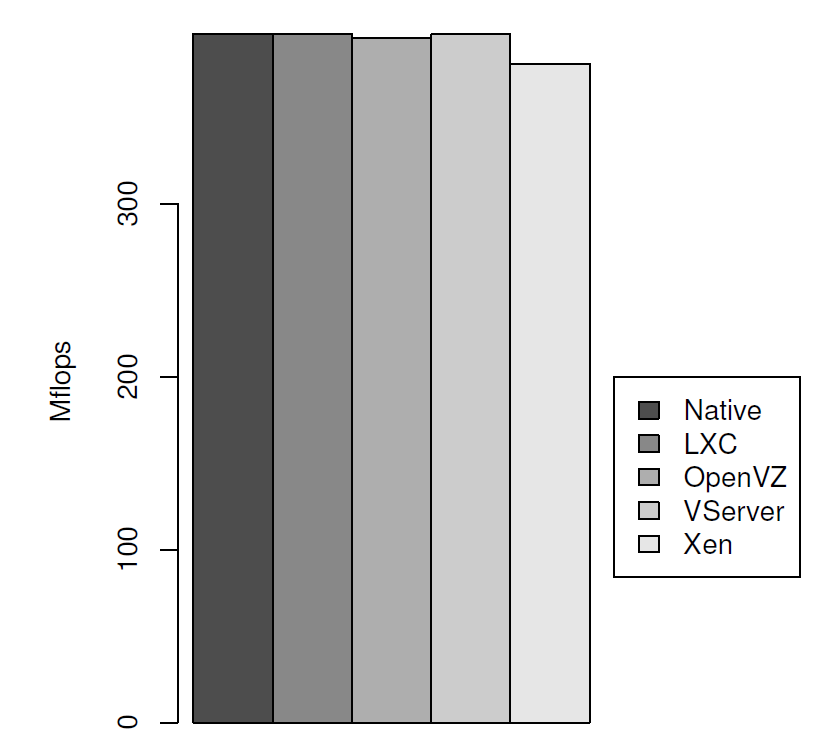
\includegraphics[width=\textwidth]{img/cpu_perf_linpack.png}
			\end{block}
		\end{column}
		\begin{column}{.5\textwidth}
			\begin{block}{\centering \textbf{Mem throughput} \\ Stream}
				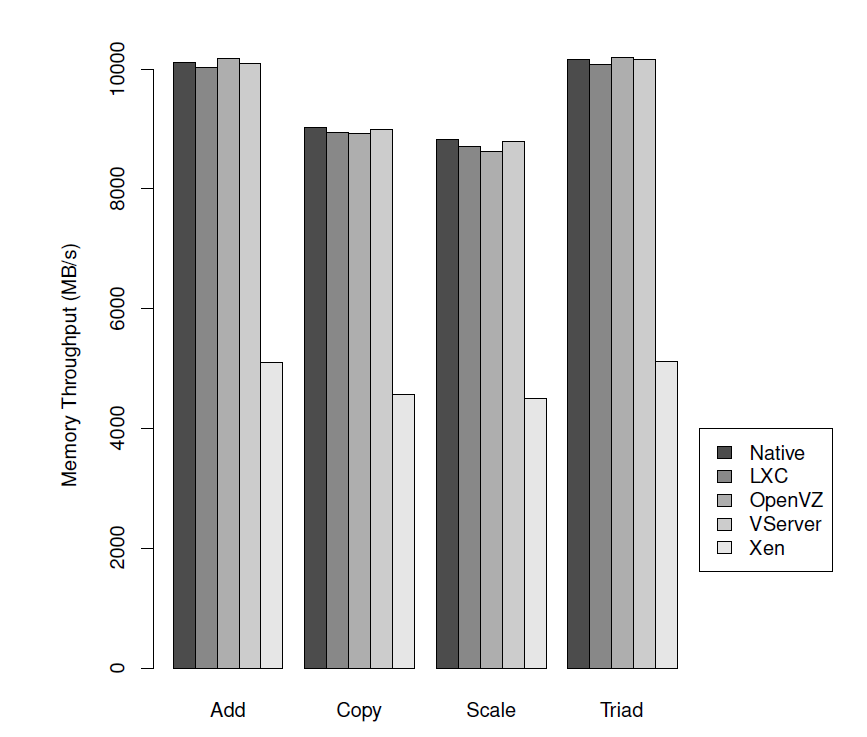
\includegraphics[width=\textwidth]{img/mem_throughput_stream.png}
			\end{block}
		\end{column}
	\end{columns}
\end{frame}

\begin{frame}{Networking Performance}
	\begin{columns}[T]
		\begin{column}{.5\textwidth}
			\begin{block}{\centering \textbf{Bandwidth} \\ NetPIPE}
				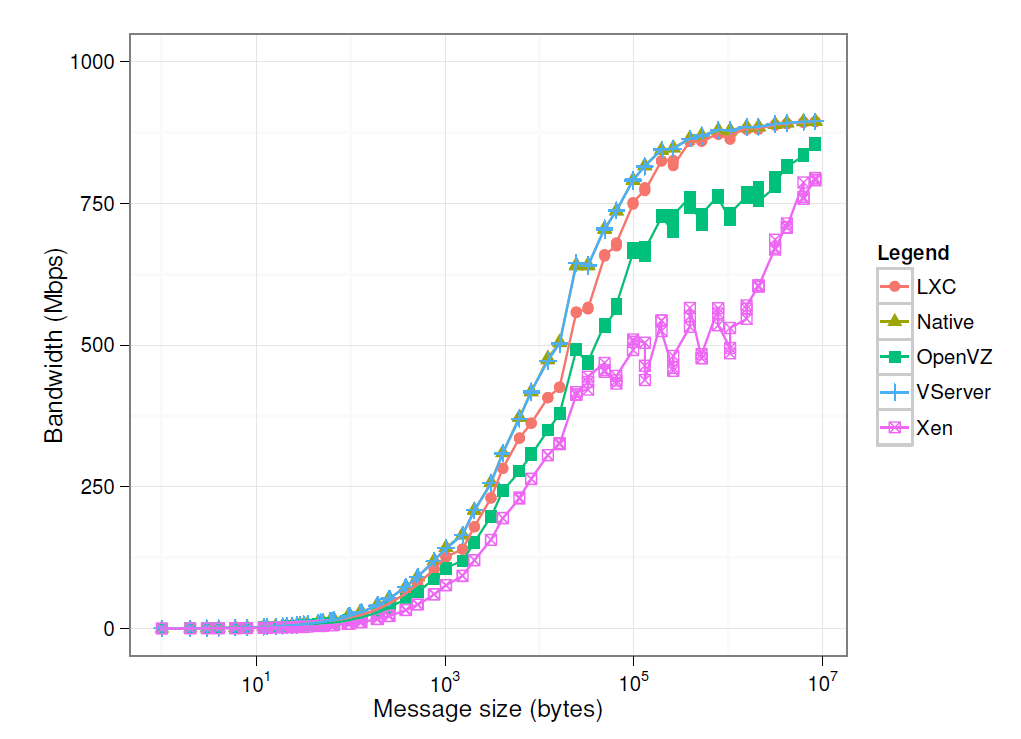
\includegraphics[width=\textwidth]{img/net_bandwidth_netpipe.png}
			\end{block}
		\end{column}
		\begin{column}{.5\textwidth}
			\begin{block}{\centering \textbf{Latency} \\ NetPIPE}
				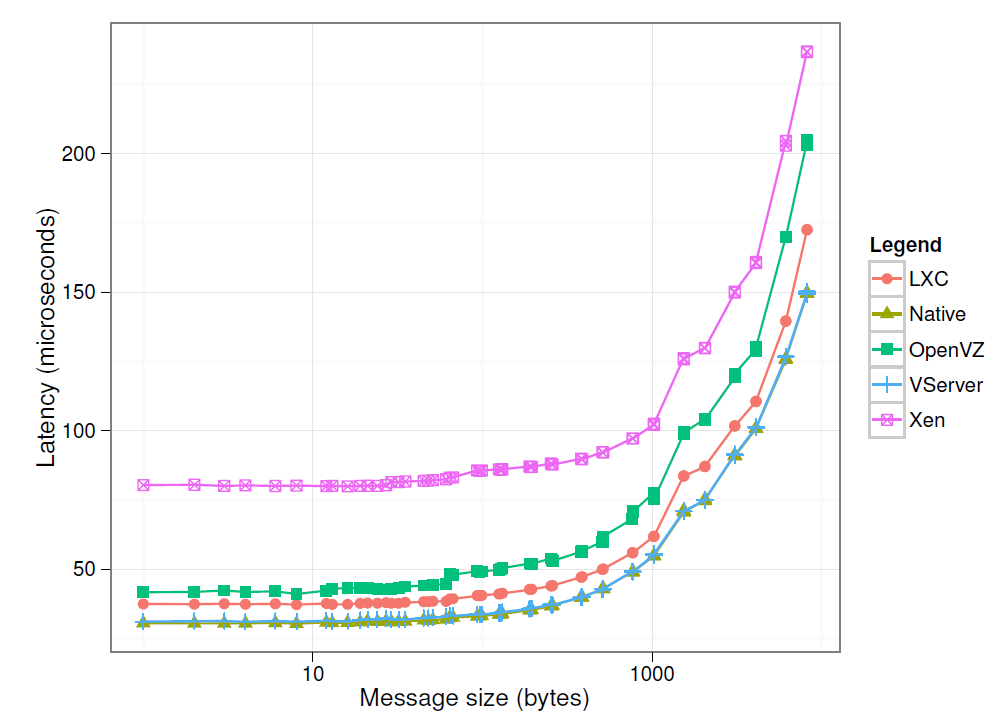
\includegraphics[width=\textwidth]{img/net_latency_netpipe.png}
			\end{block}
		\end{column}
	\end{columns}
\end{frame}

\begin{frame}{Isolation}
	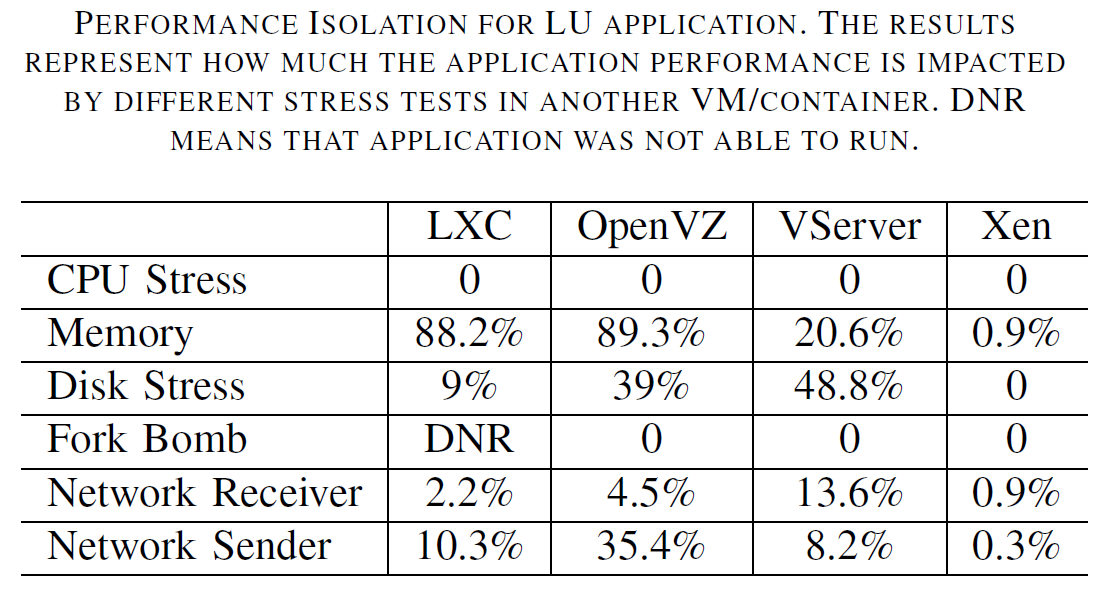
\includegraphics[width=\textwidth]{img/isolation_benchmark_suite.png}
\end{frame}


\end{document}
